\chapter{Evaluation}
% \begin{itemize}
%   \item Were the requirements correctly identified? 
%   \item Were the design decisions correct?
%   \item Could a more suitable set of tools have been chosen?
%   \item How well did the software meet the needs of those who were expecting to use it?
%   \item How well were any other project aims achieved?
%   \item If you were starting again, what would you do differently?
% \end{itemize}

\begin{figure}
\centering
\begin{verbatim}
------------------------------------------------------------------
Language      files          blank        comment           code
------------------------------------------------------------------
C                 7            233            174           1341
C/C++ Header     10            141            100            521
C++               4             68             43            246
CMake             4             22             15             60
------------------------------------------------------------------
SUM:             25            464            332           2168
------------------------------------------------------------------
\end{verbatim}
\caption[Project statistics]{The project source code at the time of submission contains 130 commits on 2168 lines of code primarily written in C.}
\label{fig:my_label}
\end{figure}

\section{Design Reflection}
The initial design of the application at the time was mostly adequate for the project. The structure of the program closely resembles what was planned in figure~\ref{overall_architecture}. It differs from the end result (See figure~\ref{fig:dependency_graph}) in the use of some utility files such as ``log.h'' and the standard lib includes. 

Greater research and design for the process of receiving and processing packets into the system could have been made. While the current system is adequate, its functions have to account for reading slightly delayed packets from the application buffer. This component of the system should be more efficient, as actions of the library will be expected to be as fast as possible, especially if the action is linked to a simple button in a GUI application.

\begin{figure}[h!]
    \centering
    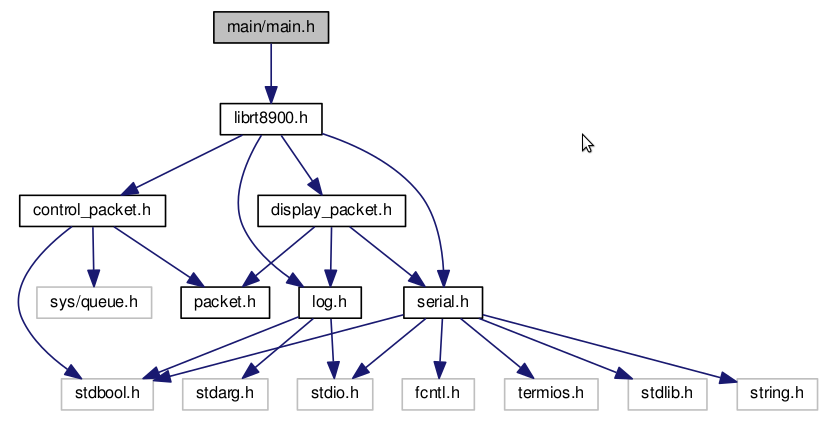
\includegraphics[width=1\textwidth]{img/dependancy_graph.png}
    \caption[Dependency graph]{Graph of the entire application dependency tree. This includes all standard library usages. The graph differs from the designed architecture in the use of a number of utility files such as serial.h and log.h}
    \label{fig:dependency_graph}
\end{figure}

\section{Suitability of tools}
\subsection*{C}
C was the best choice for this project in order to work as closely with data structures and serial interfaces. The relatively small size and low use of strings in the project contributed to the suitability of using the C language. Initially, unit tests with C++ prohibited certain C11 functions, however this was remedied with proper library linking. Compilation was exceedingly quick. Tools where always included directly in Linux distribution package managers unlike many other languages such as Python that use their own. 

\subsection*{Jenkins}
Using Jenkins over some of the free online platforms was a superior choice as it provided a better amount of customisation for the builds. For example, the build was able to use executables such as Cppcheck and GCC from the host system. Using a dedicated system over a service gave faster builds as well as more reliable time metrics so the build time could be monitored effectively.

\subsection*{Git}
Even for a single developer, the use of git helped maintain changes between computers. Fixes could occur in the lab while new features could be simultaneously developed on a separate branch for easy merges later. This helped fuel the ability to make quick changes without fear of versioning problems. The commit log helped to document changes, helping to review iterations for the blog posts as well as for this report. 

\section{Improvements}

After the second iteration, the length of iteration cycle could have been shortened from the two week period down to one. This was evident in the later iterations, as these contained many more features, therefore they could be shortened so that the iterations remained more focused. A reduction down to a single week iteration was mistakenly forgone for the sake of consistency of iteration lengths. 

The \gls{cli} was an expected feature, however it was an oversight to not provide an overall design for it. Stories and acceptance tests could have been made for these at the beginning of the project. This resulted in significant re-factoring in the last iteration in order to improve the overall code quality and maintainability of the shell. Better research and planning of a \gls{cli} as well as the the display packet reading thread earlier would have avoided difficulty in determining the testing latency later.

It was found out later that the targeted radio was the FT-8900r has a number of variants for each region. This is a problem as these models differ in their allowed frequencies for transmission. Currently only the Europe version is properly supported, with the US and Asia regions missing their configuration. This was a problem as it was difficult to source the frequency lists. In the future the likely solution would to have a number of lists for transmission that can be chosen via an optional flag to choose the model at runtime.

Unit tests were written primarily for library functions that manipulated packets. Testing of the actual user interface by capturing input and output of the program may have been a useful automation in order to decrease the time spent testing. During implementation this was not a priority due to how quick manual testing to the same end was. It can be foreseen however, that this would become more difficult in the future, as more and more features are added to the project.

The most useful development in the future would be to add an inter process communication method. The user shell would be moved out to a separate client that would talk to the server via a socket. This would allow other applications to utilise the socket \gls{8900} control such as Hamlib with a small patch. This would also permit making the \gls{cli} in another language, which may have facilitated faster development.

\section{Objectives}

\begin{table}[H]
\centering
\begin{tabular}{l|l}
Objective & Status \\
\hline
Final report & Complete \\
Frequency & Complete \\
Push to talk & Complete \\
Volume & Complete \\
Squelch & Complete \\
Power & Complete \\
Powering on the radio & Partial (Completed in software) \\
Code documentation & Complete \\
Schematic & Complete
\end{tabular}
\caption{List of objectives/deliverables}
\label{table:objectives}
\end{table}

It is the opinion of the developer that the project aims have been met. Users of the application have been provided with a useful, portable and fast application to control their \gls{8900} radios without the high cost of existing solutions. The hardware requirement of turning on the radio was only partially met. However a remote shack could still easily leave their radio on, ready for transmission (the radio will not consume much power when idle). For audio the data port at the back of the radio already provides this function. A good experience for a remote shack operator can be made with the use of a VOIP application such as Mumble~\cite{mumble} for audio and SSH to control the project application.